\hypertarget{base64}{%
\subsection{base64}\label{base64}}

Base64 是一种用 64 个字符来表示任意二进制数据的方法。

用记事本打开\texttt{exe}、\texttt{jpg}、\texttt{pdf}这些文件时,我们都会看到一大堆乱码,因为二进制文件包含很多无法显示和打印的字符,所以,如果要让记事本这样的文本处理软件能处理二进制数据,就需要一个二进制到字符串的转换方法。Base64
是一种最常见的二进制编码方法。

Base64 的原理很简单,首先,准备一个包含 64 个字符的数组:

\begin{pythoncode}
['A', 'B', 'C', ... 'a', 'b', 'c', ... '0', '1', ... '+', '/']
\end{pythoncode}

然后,对二进制数据进行处理,每 3
个字节一组,一共是\texttt{3x8=24}bit,划为 4 组,每组正好 6 个 bit:

 
 \begin{figure}[htp]
	\centering
	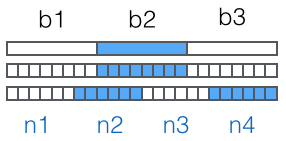
\includegraphics[width=0.6\linewidth]{fig/949444125467040.png}
\end{figure}


这样我们得到 4 个数字作为索引,然后查表,获得相应的 4
个字符,就是编码后的字符串。

所以,Base64 编码会把 3 字节的二进制数据编码为 4
字节的文本数据,长度增加
33\%,好处是编码后的文本数据可以在邮件正文、网页等直接显示。

如果要编码的二进制数据不是 3 的倍数,最后会剩下 1 个或 2
个字节怎么办?Base64
用\texttt{\textbackslash{}x00}字节在末尾补足后,再在编码的末尾加上 1
个或 2 个\texttt{=}号,表示补了多少字节,解码的时候,会自动去掉。

Python 内置的\texttt{base64}可以直接进行 base64 的编解码:

\begin{pythoncode}
>>> import base64
>>> base64.b64encode(b'binary\x00string')
b'YmluYXJ5AHN0cmluZw=='
>>> base64.b64decode(b'YmluYXJ5AHN0cmluZw==')
b'binary\x00string'
\end{pythoncode}

由于标准的 Base64 编码后可能出现字符\texttt{+}和\texttt{/},在 URL
中就不能直接作为参数,所以又有一种 ``url safe'' 的 base64
编码,其实就是把字符\texttt{+}和\texttt{/}分别变成\texttt{-}和\texttt{\_}:

\begin{pythoncode}
>>> base64.b64encode(b'i\xb7\x1d\xfb\xef\xff')
b'abcd++//'
>>> base64.urlsafe_b64encode(b'i\xb7\x1d\xfb\xef\xff')
b'abcd--__'
>>> base64.urlsafe_b64decode('abcd--__')
b'i\xb7\x1d\xfb\xef\xff'
\end{pythoncode}

还可以自己定义 64 个字符的排列顺序,这样就可以自定义 Base64
编码,不过,通常情况下完全没有必要。

Base64
是一种通过查表的编码方法,不能用于加密,即使使用自定义的编码表也不行。

Base64 适用于小段内容的编码,比如数字证书签名、Cookie 的内容等。

由于\texttt{=}字符也可能出现在 Base64 编码中,但\texttt{=}用在
URL、Cookie 里面会造成歧义,所以,很多 Base64 编码后会把\texttt{=}去掉:

\begin{pythoncode}
'abcd' -> 'YWJjZA=='

'abcd' -> 'YWJjZA'
\end{pythoncode}

去掉\texttt{=}后怎么解码呢?因为 Base64 是把 3 个字节变为 4
个字节,所以,Base64 编码的长度永远是 4
的倍数,因此,需要加上\texttt{=}把 Base64 字符串的长度变为 4
的倍数,就可以正常解码了。

\hypertarget{ux5c0fux7ed3}{%
\subsubsection{小结}\label{ux5c0fux7ed3}}

Base64 是一种任意二进制到文本字符串的编码方法,常用于在
URL、Cookie、网页中传输少量二进制数据。

\hypertarget{ux7ec3ux4e60}{%
\subsubsection{练习}\label{ux7ec3ux4e60}}

请写一个能处理去掉\texttt{=}的 base64 解码函数:

\begin{pythoncode}
# -*- coding: utf-8 -*-
import base64
\end{pythoncode}

\begin{pythoncode}
# 测试:
assert b'abcd' == safe_base64_decode(b'YWJjZA=='), safe_base64_decode('YWJjZA==')
assert b'abcd' == safe_base64_decode(b'YWJjZA'), safe_base64_decode('YWJjZA')
print('ok')
\end{pythoncode}

\hypertarget{ux53c2ux8003ux6e90ux7801}{%
\subsubsection{参考源码}\label{ux53c2ux8003ux6e90ux7801}}

\href{https://github.com/michaelliao/learn-python3/blob/master/samples/commonlib/do_base64.py}{do\_base64.py}

